\documentclass[tikz,border=0pt]{standalone}
\usepackage{graphicx}
\usepackage{helvet}
\renewcommand{\familydefault}{\sfdefault}
\begin{document}
\begin{tikzpicture}[x=1mm,y=1mm]
  \node[anchor=south west,inner sep=0] at (0,0)
    {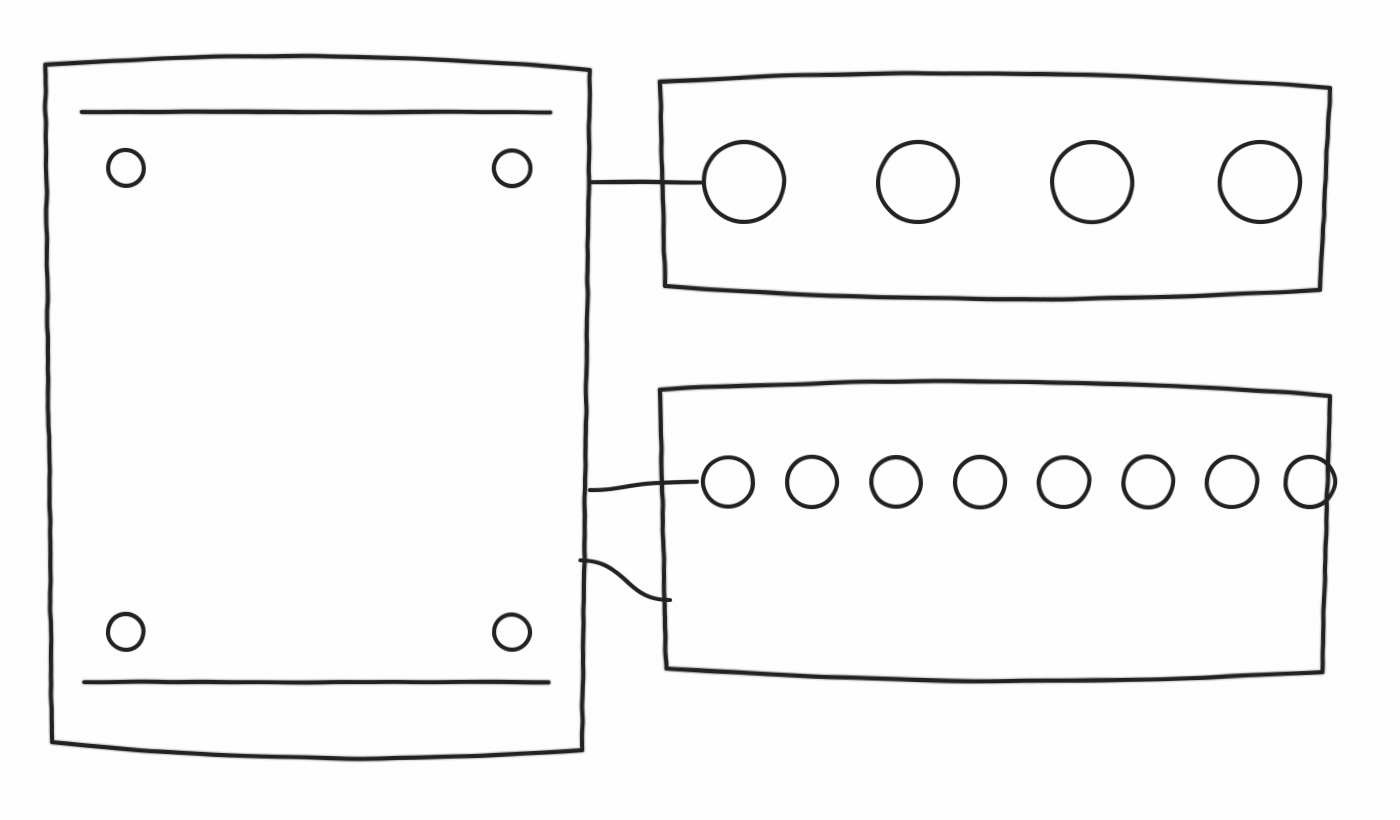
\includegraphics[width=140mm,height=82mm]{028-inert-channel-pencil-base.png}};
  \node[font=\bfseries\large] at (31.8,72.2) {MEGA 2560};
  \node[font=\scriptsize] at (20,60) {USB POWER ONLY};
  \node[font=\scriptsize] at (23,54) {D30--D33 pull-up buttons};
  \node[font=\scriptsize] at (22,48) {D22--D29 through 1 kOhm to LED};
  \node[font=\scriptsize] at (20,42) {each LED cathode to GND};
  \node[font=\scriptsize] at (20,34) {TP28: selected button pin};
  \node[font=\scriptsize] at (19,28) {TP29: indicator output};
  \node[font=\bfseries\small] at (99,69)
    {LEARNER-OPERATED SYNTHETIC INPUTS};
  \node[font=\scriptsize] at (74.5,56.5) {CHANNEL};
  \node[font=\scriptsize] at (91.8,56.5) {PRIMARY};
  \node[font=\scriptsize] at (109.2,56.5) {REDUNDANT};
  \node[font=\scriptsize] at (126,56.5) {APPLY};
  \node[font=\bfseries\small] at (99,38.5) {EIGHT INERT CHANNEL INDICATORS};
  \foreach \x/\n in {72.8/0,81.2/1,89.6/2,98/3,106.4/4,114.8/5,123.2/6,131/7}
    \node[font=\scriptsize] at (\x,27.2) {\n};
  \node[font=\scriptsize] at (99,20)
    {assessment to cadence; no external-load connection};
  \node[font=\scriptsize] at (70,2)
    {Orientation plate: verify exact pins unpowered against the canonical sketch.};
\end{tikzpicture}
\end{document}
